% Brian Mc George - MCGBRI004
% Jacques Heunis - HNSJAC003
% Timothy Gwynn - GWNTIM001
% Due: 31-07-2015
% Stage One - Software Engineering  - CSC3003S
\documentclass[a4paper,10pt]{article}
%**************************************************************************************************
% PACKAGES
%**************************************************************************************************
\usepackage{amsmath, amsthm, amsfonts, amssymb}
\usepackage{graphicx,color}
\usepackage{bm}	
\usepackage{float}
\usepackage{caption, subcaption}
%\usepackage{vector}

%**************************************************************************************************
% DEFAULT SETTINGS
%**************************************************************************************************
\marginparwidth -20 true pt    % Width of marginal notes.
\oddsidemargin  -10 true pt       % Note that \oddsidemargin=\evensidemargin
\evensidemargin -10 true pt
\topmargin -0.5 true in        % Nominal distance from top of page to top of
\textheight 9.75 true in         % Height of text (including footnotes and figures)
\textwidth 7 true in        % Width of text line.
\parindent=10pt                  % Do not indent paragraphs
\parskip= 1 ex
\columnseprule = 0.1pt
\footskip = 30 true pt
\hoffset = -0.1 true in
\voffset = -0.1 true in
\abovedisplayskip 1 true pt
\abovedisplayshortskip 1 true pt
\topsep 0 true pt
\newcommand*\varhrulefill[1][0.4pt]{\leavevmode\leaders\hrule height#1\hfill\kern0pt}

%**************************************************************************************************
% DOCUMENT DETAILS
%**************************************************************************************************


%**************************************************************************************************
% MAIN DOCUMENT 
%**************************************************************************************************

\begin{document}
\begin{titlepage} \begin{center} 
		\textsc{\LARGE University of Cape Town}
		\\[1.5cm] \textsc{\Large Software Engineering Stage Two\\CSC3003S}
		\\[0.5cm]
		\noindent\rule[0.4mm]{\textwidth}{0.1mm}
		\\[0.4cm] { \huge \bfseries Tempest Trace \\[0.4cm] }
		\noindent\rule[0.4mm]{\textwidth}{0.1mm}
		\\[1cm]
		\begin{minipage}[t]{0.4\textwidth}
		\begin{flushleft}\large \emph{Authors:}\\ Brian Mc George - MCGBRI004 \\ Jacques Heunis - HNSJAC003 \\ Timothy Gwynn - GWYTIM001\end{flushleft}
		 \end{minipage} \begin{minipage}[t]{0.4\textwidth} 
		\begin{flushright} \large \emph{Supervisor:} \\ Assoc. Prof.~Patrick Marais\\patrick@cs.uct.ac.za\end{flushright}
		\begin{flushright} \large \emph{Tutor:} \\ Codie Roelf\\Codie.Roelf@alumni.uct.ac.za\end{flushright}
		 \end{minipage} \vfill {\large \today}
		\end{center}
		\end{titlepage}
\newpage
\tableofcontents
\newpage

\section{Use Case Narratives}

\section{Analysis Class Model}
\begin{figure}[H]
	\begin{center}
		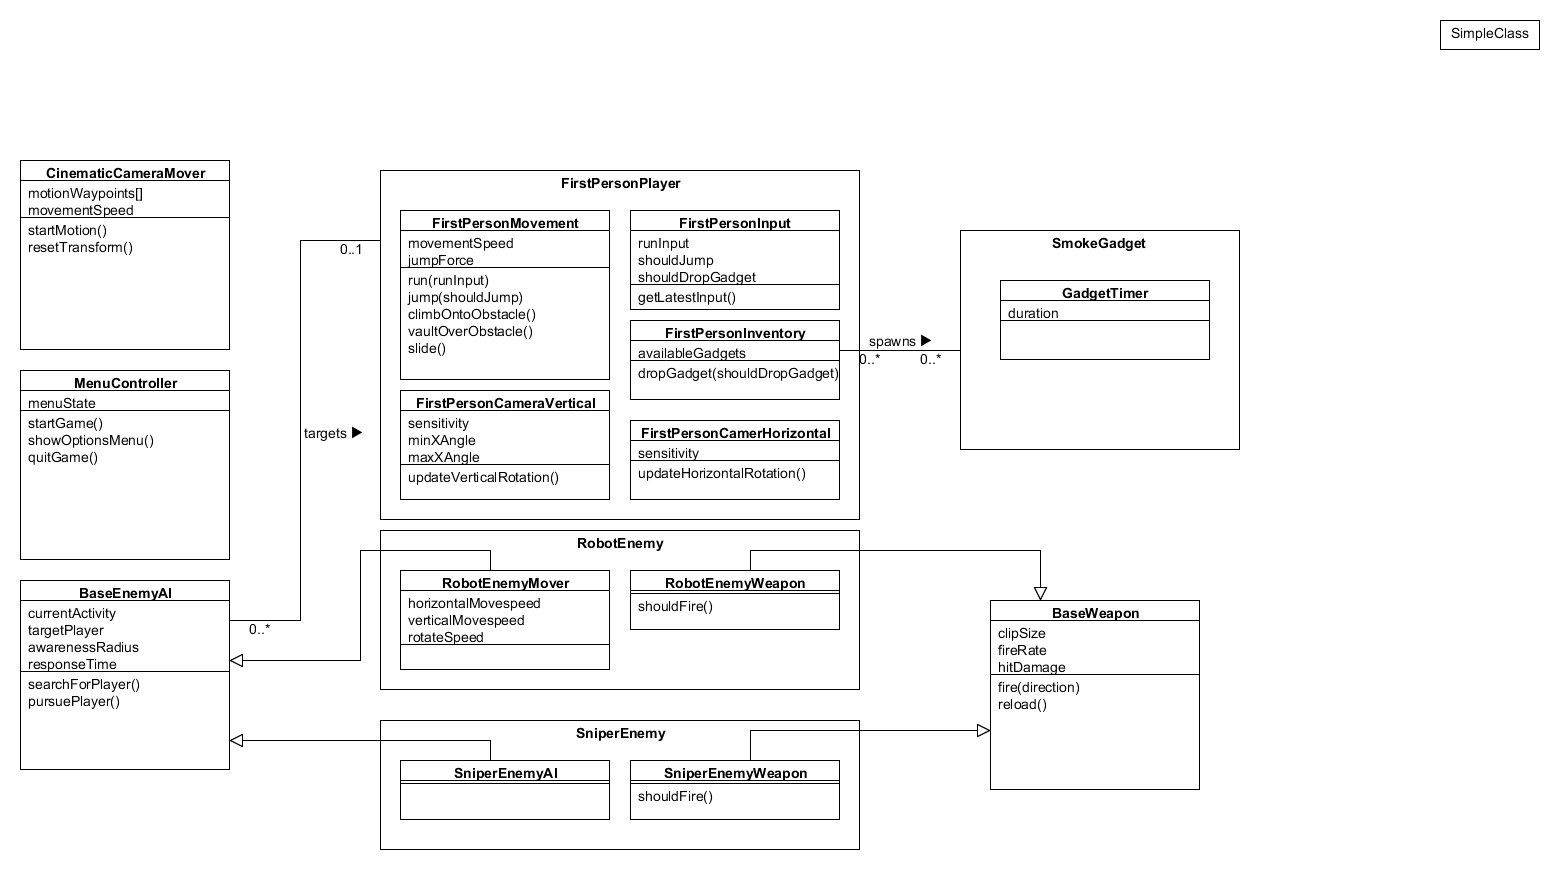
\includegraphics[scale=0.4]{images/AnalysisClassDiagram.png}
		\caption{Get analysisized!}
	\end{center}
\end{figure}
A first-draft analysis class model.

\section{State Diagrams}
\begin{figure}[H]
	\begin{center}
		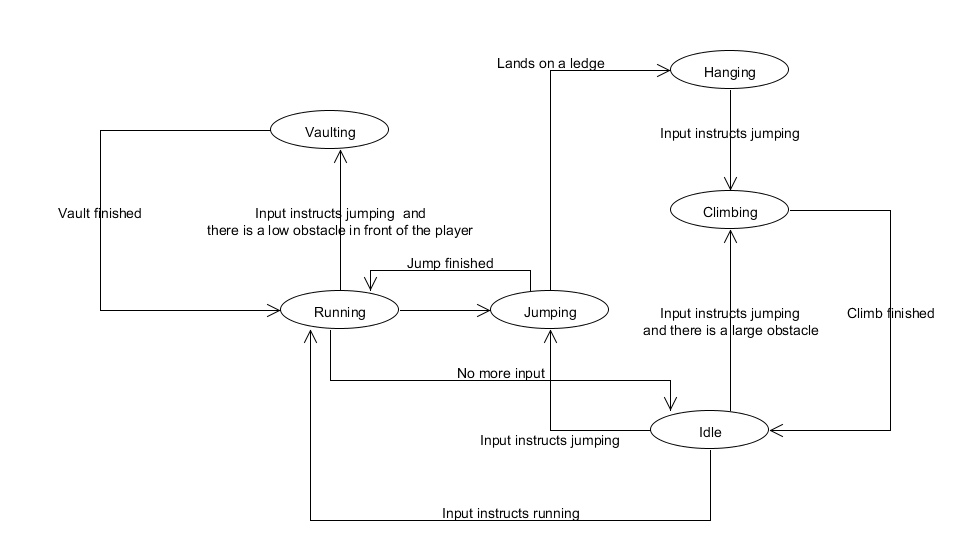
\includegraphics[scale=0.4]{images/PlayerStateMachine.png}
		\caption{A state machine for the player}
	\end{center}
\end{figure}
\begin{figure}[H]
	\begin{center}
		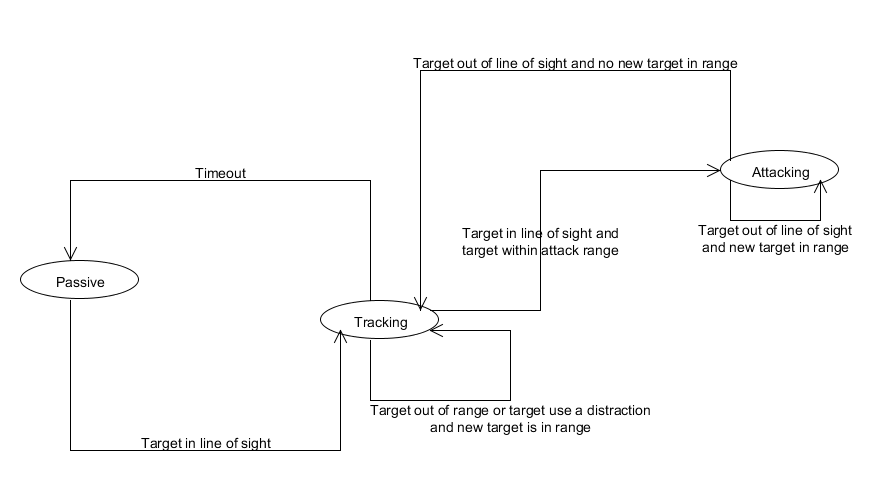
\includegraphics[scale=0.4]{images/EnemyStateMachine.png}
		\caption{A state machine for the 2 types of enemies in the game}
	\end{center}
\end{figure}

\section{Project Plan}

\section{Test Plan}
    \subsection{Game ends when player reaches finish line}
        \textbf{Pre-conditions}\\
        Both players have not passed the finish line. 
        \smallskip\\\textbf{Input}\\
        A player passes the finish line.
        \smallskip\\\textbf{Expected output}\\
        The game timer stops and the end game screen is shown.
        
    \subsection{Player jumps forward}
        \textbf{Pre-conditions}\\
        Player is moving and no obstacle within half a metre in front of player. 
        \smallskip\\\textbf{Input}\\
        A player presses the jump button.
        \smallskip\\\textbf{Expected output}\\
        The player jump animation plays and the player moves both forward and upwards. 
        
    \subsection{Player climbs up ledge}
    \textbf{Pre-conditions}\\
    Obstacle is within half a metre and its height within a range of 1.5 metres to 2 metres in front of player. 
    \smallskip\\\textbf{Input}\\
    A player presses the jump button.
    \smallskip\\\textbf{Expected output}\\
    The player climb animation plays and the player moves upwards onto the obstacle.
    
    \subsection{Player vaults over obstacle}
    \textbf{Pre-conditions}\\
    Player is moving. Obstacle is within half a metre and its height is less than 1.5 metres in front of player. 
    \smallskip\\\textbf{Input}\\
    A player presses the jump button.
    \smallskip\\\textbf{Expected output}\\
    The player vault animation plays and the player moves onto the top of the obstacle.
    
    \subsection{Smoke bomb deployed}
    \textbf{Pre-conditions}\\
    Player has smoke bombs remaining.
    \smallskip\\\textbf{Input}\\
    A player presses the smoke bomb button.
    \smallskip\\\textbf{Expected output}\\
    The player smoke bomb throw animations plays and the bomb is thrown to the ground. When the bomb reaches the ground, a small explosion occurs and a smoke cloud covers the area.
    
    \subsection{Sniper hits player}
    \textbf{Pre-conditions}\\
    Player is tracked by sniper. Player is not moving.
    \smallskip\\\textbf{Input}\\
    No input from player.
    \smallskip\\\textbf{Expected output}\\
    The player is shot by the sniper after two seconds.
    
    \subsection{Sniper does not hit player}
    \textbf{Pre-conditions}\\
    Player is tracked by sniper. Player is moving at running velocity.
    \smallskip\\\textbf{Input}\\
    Player stays moving.
    \smallskip\\\textbf{Expected output}\\
    The sniper misses 66\% of shots at player.
    
    \subsection{Drone tracks player}
    \textbf{Pre-conditions}\\
    Player within line of sight of drone. Player within 50 metres from drone. Drone is not tracking a player already.
    \smallskip\\\textbf{Input}\\
    Player stays in vision of drone for at least one second.
    \smallskip\\\textbf{Expected output}\\
    The drone tries to get within range to fire at player. The drone fires at the player when within range.
        
\end{document}
